\chapter{Microservices}

Der Begriff Microservices stifte derzeit noch große Verwirrung. Nicht nur weil er relativ neu ist, sondern auch weil er sehr breit gefächert ist und eine klare Abgrenzung kaum möglich ist. Im nachfolgenden Kapitel wird der Begriff Microservice ausführlich definiert, beschrieben und zu anderen Konzepten abgegrenzt.

\section{Was ist ein Microservice}

Hinter Microservices verbirgt sich keine Technologie die aktiv entwickelt wurde. Vielmehr ist es ein Sammelbegriff der nachträglich für über die Jahre entstandener Praktiken, Methoden und Technologien, im Umfeld von komplexen Softwaresystemen, eingeführt wurde. Am häufigsten ist mit Microservices die sogenannte Microservice Architektur gemeint. Charakteristisch für dieses Softwarearchitekturmuster ist die Zerlegung eines Softwaresystems in kleine, autonome Dienste, die mit einem leichtgewichtigem Kommunikationsprotokoll miteinander interagieren, zu einem zu einem verteilten System. Die Fähigkeiten eines einzelnen Dienstes ist genau auf die Geschäftsanforderungen eines bestimmten Unternehmens oder Einsatzgebietes zugeschnitten \cite{FowlerMS}. Die Verwendung dieses Muster bringt aber neben technischen Einflüssen, meistens auch organisatorische Einflüsse mit sich. Beispielsweise auf die Teamstruktur, Verantwortung, Continuous Integration, Testing, um nur einige davon zu nennen. Daher können mit den Begriff Microservices viele verschiedene Aspekte gemeint sein.

Um zu verstehen warum sich Microservices derart großer Beliebtheit erfreuen, ist es notwendig zu verstehen, wie die Architektur derartiger Systeme vor diesem Paradigmenwechsel ausgesehen hat. Dazu beschreibt der nächste Abschnitt den sogenannten monolithischen Ansatz und welche Probleme damit verbunden sind, die durch Microservices gelöst werden.

\subsection{Monolithische Ansatz}

Mittlerweile haftet der monolithischen Softwarearchitektur, zu unrecht, ein negativer Ruf an. Obwohl dieser Ansatz seit Jahrzehnten  in vielen Bereichen der Softwareindustrie sehr gut funktioniert. Im Java und .NET Umfeld war \bzw ist dieser Ansatz noch immer gängige Praxis. Dennoch wird er vielerorts von der Microservice Architektur abgelöst. Doch was macht eine Anwendung überhaupt zu einem Monolithen?

Unter einem Monolithen versteht man in der Softwareentwicklung eine Anwendung, in der verschiedene Geschäftsbereiche oder Funktionalitäten als eine einzige Anwendung zusammengeschlossen sind \cite{FowlerMS}. Intern kann die Applikation beispielsweise als Mehrschicht-Architektur organisiert sein. Üblich sind hier folgende drei Schichten \cite{FowlerPEA}:

\begin{itemize}
	\item \textbf{Präsentationsschicht:} Hier ist derjenige Quelltext angesiedelt, der sich mit der Darstellung der Benutzerschnittstelle, \zB als Web- oder Desktopanwendung auseinandersetzt.
	\item \textbf{Geschäftslogikschicht:} Diese Schicht stellt den Kern der Anwendung dar. Sie enthält alle Geschäftsrelevanten Funktionen.
	\item \textbf{Datenzugriffsschicht}: In dieser Schicht befinden sich die Funktionalität die zum Zugriff auf externen Datenquellen, wie \zB relationale Datenbanken, notwenidg ist.
\end{itemize}


In Abbildung \ref{fig:layered-architecture} ist der Aufbau eines Monolithen mit Drei-Schicht-Architektur skizziert. Der Zugriff darf jeweils nur auf die direkt darunterliegende Schicht erfolgen. Innerhalb jeder Schicht ist eine Modularisierung in verschiedene Bereiche, die auf die Geschäftsfunktionen abgestimmt sind, sinnvoll.

\begin{figure}[!htb]
\centering
\minipage{0.5\textwidth}
  \centering
	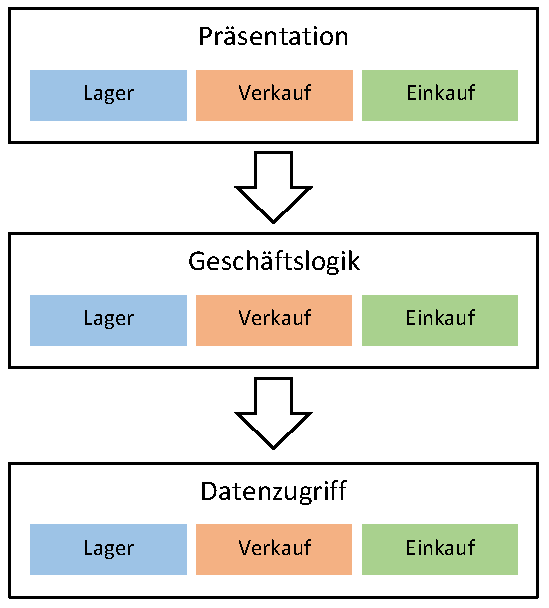
\includegraphics[width=0.8\linewidth]{layered-architecture}
	\caption{Drei-Schicht-Architektur}
	\label{fig:layered-architecture}
\endminipage
\minipage{0.5\textwidth}
  \centering
	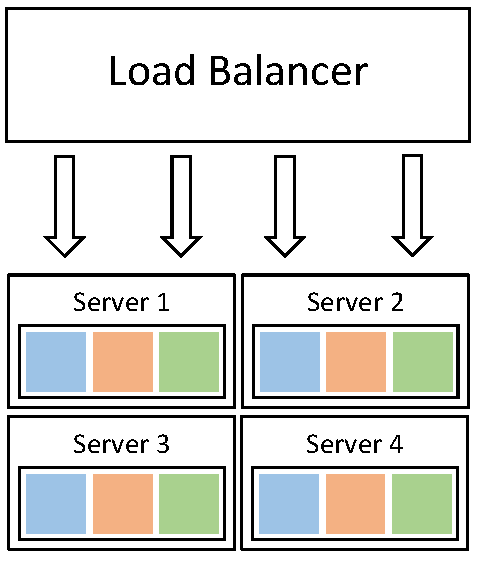
\includegraphics[width=0.76\linewidth]{monolith-scale}
	\caption{Skalieren eines Monolithen}
	\label{fig:monolith-scale}
\endminipage
\end{figure}

\subsubsection{Nachteile}

Mit steigender Komplexität kommen nach und nach Probleme zum Vorschein, der diesen Ansatz aufwändig oder sogar unpraktikabel machen. Eines der Hauptprobleme ist bei Internetweiten Anwendungen die Skalierbarkeit. Die einzige Möglichkeit einen Monolithen zu skalieren ist auf mehreren Servern jeweils eine Instanz des Monolithen zu installieren und über einen Load-Blancer zu verbinden. Abbildung \ref{fig:monolith-scale} zeigt wie ein solcher Aufbau aussehen kann. In vielen Einsatzgebieten ist dieser Ansatz aber nicht feingranular genug. Oft ist es sinnvoller nur bestimmte Teile es Gesamtsystems zu skalieren.

Ein Monolith stößt aber nicht nur aus technischer Sichtweise auf Skalierbarkeitsprobleme, sondern auch aus organisatorischer Sicht. Alle Entwickler arbeiten zwangsläufig an der gleichen Codebasis, die dadurch enorme Größe annehmen kann. Kein einzelner Entwickler ist mehr in der Lage die ganze Codebasis zu überblicken und zu beurteilten welche Auswirkung eine Änderung haben kann. Das führt über kurz oder lang zur Verlangsamung der Entwicklungsgeschwindigkeit oder sogar zu völligem Stillstand.

Vor allem in Technologiebranche ändern sich Anforderungen sehr rasch. Agile Softwareprozesse unterstützen dabei, die geänderten Anforderung so schnell es geht in die Software einfliessen zu lassen. Für den Kunden \bzw Endbenutzer zählt nur die schnellstmögliche Umsetzung seiner neuen Anforderungen. In einem Monolithen sind mehrere Geschäftsbereiche zusammengefasst. Der Monolith muss immer als ganzes getestet und ausgerollt werden. Dadurch verlangsamt sich der gesamte Releasezyklus auf den langsamsten Teilbereich, obwohl vielleicht der Teilbereich in dem eine Änderung notwendig war, schon längst fertiggestellt ist.

Hinter einem Monolith steht immer eine bestimmte Technologie oder eine Sammlung von mehreren Technologien, wie \zB Java EE oder ASP.NET. Somit müssen alle Teilbereiche der Anwendung auf die selben Technologien zurückgreifen. Für manche Teilbereiche könnte aber möglicherweise die Verwendung von alternativen Technologien und Speichersystemen große Vorteile bringen.

In diesem Abschnitt wurden einige der Hauptkritikpunkte am monolithischen Architekturmuster angeführt. Es mag den Anschein vermittelt haben, dass dieser Ansatz nicht mehr verwendet werden soll. Im Gegenteil. Viele Experten sind der Meinung, dass gerade am Anfang eines Projekts der monolithische Ansatz zu bevorzugen ist \cite{FowlerMolithFist}. Erst nachdem das Verständnis für die Domäne vorhanden ist und Anforderungen klarer sind, ist der Übergang zu einer Microservice Architektur leichter und sinnvoll. 

\section{Charakteristiken eines Microservice}

Dieser Abschnitt beschreibt einige charakteristische Merkmale eines Microservice. Wie bereits erwähnt gibt es keine eindeutige Definition eines Microservice. Daher sind auch in der Literatur sehr viele unterschiedliche Merkmale von Microservices zu finden. Die nachfolgenden Charakteristiken beruhen großteils auf \cite{HorsdalMS} und \cite{FowlerMS}.

\subsection{Prinzip der eindeutigen Verantwortlichkeit}

In der sauberen objektorientierten Programmierung ist das Prinzip der eindeutigen Verantwortung längst fester Bestandteil \cite{MartinAgile}:

\begin{english}
\begin{quote}
  \textit{A class should have only one reason to change.}
\end{quote}
\end{english}

Im Kontext von Microservice wird dieser Grundsatz von der Klassen-Ebenen auf die Dienst-Ebene erweitert. Das heißt für jeden Dienst soll genau eine Fähigkeit realisieren. Damit ist sichergestellt, dass geänderte Geschäftsanforderungen so wenig Dienste wie notwendig beeinflussen.

\subsection{Ausrollen pro Dienst}

Um von den Vorteilen der Microservice Architektur gegenüber eines Monolithen profitieren zu können, ist es unabdingbar, dass jeder Dienst einzeln ausgerollt werden kann. Denn nur damit sind die Entwicklungs- und Releasezyklen der einzelnen Dienste im Gesamtsystem voneinander Unabhängig.

Wenn jeder Dienst einzeln ausgerollt werden kann, ist es auch möglich, unterschiedliche Versionen diese Dienst auszurollen. Somit kann einen neue Version getestet werden und erst wenn diese Testphase erfolgreich war der gesamte Datenverkehr auf diesen Dienst umgeleitet werden. Bei Problemen kann schnell der ursprüngliche Zustand wiederhergestellt werden. Insgesamt mindert ein derartiges Vorgehen das Risiko eines großen Deployments.

Damit dieser Ansatz funktioniert, müssen die Dienste einige Anforderungen erfüllen. Jeder Dienst steht mit einigen anderen in Verbindung. Wenn nun eine neue Version eines Dienst ausgerollt wird, muss dessen Schnittstelle Abwärtskompatibel sein, da seine Konsumenten die alte Schnittstelle verwenden. Fehlertoleranz ist eine weitere wichtige Eigenschaft, da während eine neue Version ausgerollt wird, der Dienst kurzzeitige nicht Verfügbar sein kann.

\subsection{Dezentrale Datenverwaltung}

Eine monolithische Applikation legt sehr häufig alle persistenten Daten in einer einzigen, \zB relationalen, Datenbank ab. In einer Microservice Architektur ist dieser Ansatz nicht mehr empfehlenswert. Jede Datentyp sollen nur von einem Dienst verwaltet werden und nicht einfach direkt von einem anderen Dienst aus der Datenbank gelesen werden. Dadurch werden die Abhängigkeiten auf ein Minimum reduziert, denn andere Dienste können nur über die Schnittstelle des bereitstellenden Dienstes Daten abfragen und manipulieren. Dieses Anti-Pattern ist noch einmal in Abbildung \ref{fig:central-datastore} verdeutlicht.

\begin{figure}[h]
  \centering
	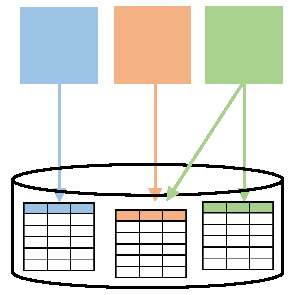
\includegraphics[width=0.3\textwidth]{central-datastore}
	\caption{Zentraler Datenspeicher}
	\label{fig:central-datastore}
\end{figure}

Wenn jeder Dienst, wie in Abbildung \ref{fig:polyglot-persistnace}, seinen eigenen Datenspeicher besitzt, kann für die Erfüllung seiner Aufgabe der optimale Speichermechanismus ausgewählt werden. Beispielsweise können Daten mit komplexen Beziehung in einer Graphendatenbank abgelegt werden. Jedoch einfache Daten in einem schnellen Key-Value-Speicher.

\begin{figure}[h]
  \centering
	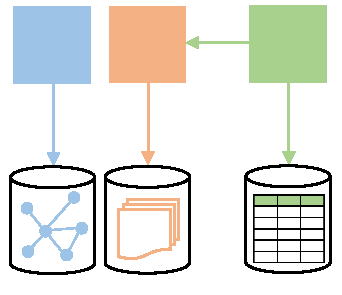
\includegraphics[width=0.3\textwidth]{polyglot-persistance}
	\caption{Polyglot Persistance}
	\label{fig:polyglot-persistnace}
\end{figure}

Auch ein Monolith könnte Gebrauch von mehreren Datenbanken machen. Dieser Ansatz ist unter dem Namen Polyglot Persistence bekannt \cite{FowlerPP}. Aus teilweise sehr vielfältigen Gründe ist er aber selten anzutreffen. Nachfolgend nur ein kleiner Auszug:

\begin{itemize}
  \item Die IT-Strategie einiger Unternehehmen sehen nur die Verwendung ganz bestimmter Datenbanken vor.
	\item Bereits getätigte Investitionen in bestehende Datenbanken müssen amortisiert werden.
	\item Angst vor dem Betrieb einer Datenbank für die noch nicht die notwendige Erfahrung aufgebaut wurde.
\end{itemize}

Für Systeme mit hohen Anforderungen an die Verfügbarkeit ist eine einige Datenbank aber kaum tragbar. Denn eine einzige Datenbank stellt einen kritischen \textit{Single Point of Failure} dar.